\documentclass[a4paper,11pt]{ctexart}
\usepackage{xcolor}
\usepackage{amsmath}
\usepackage{amssymb}
\usepackage{graphicx}
\usepackage{bookmark}
\usepackage{booktabs}
\usepackage{textcomp}
\usepackage[text={6.5in,9in},centering]{geometry}
\usepackage{hyperref}
\usepackage{bm}
\usepackage{array}
\usepackage{multirow}

\usepackage{caption}
\captionsetup{width=0.75\textwidth,font={small,sl}}

\usepackage{afterpage}

\def\blankpage{%
      \clearpage%
      \thispagestyle{empty}%
      \addtocounter{page}{-1}%
      \null%
      \clearpage}

\newcommand{\RT}[1]{\textcolor{red}{#1}}
\newcommand{\BT}[1]{\textcolor{blue}{#1}}
\newcommand{\GT}[1]{\textcolor{green}{#1}}
\newcommand{\MT}[1]{\textcolor{magenta}{#1}}

\begin{document}

%设置标题、作者
\title{巡天模拟}
\author{许优华}

\maketitle


%设置摘要
\abstract{
首先介绍模拟运行的条件以及它们的实现,然后展示根据模拟结果得到的天区覆盖图以及面积统计的结果,
接着我们尝试分析目前模拟中依然存在哪些显著影响编排结果的限制因素,以便在后续的工作中针对这些因素
进行优化。最后,附录部分列出了模拟程序运行时读取的所有参数的详细信息。}

%显示目录
\newpage
\tableofcontents


%\blankpage
%%%%%%%%%%%%%%%%%%%%%%%%%%%%%%%%%%%%%%%%%%%%%%%%%%%%%%%%%%
\section{文档简介}
本文档的目的在于记录“巡天编排模拟”工作中遇到的各项问题以及具体的解决方案。有了这些记录,可以确保
一轮一轮的优化过程中少走弯路。简单来说,这份文档应该看作是一份技术文档,额外增加了一些模拟结果的
内容。

\blankpage
%%%%%%%%%%%%%%%%%%%%%%%%%%%%%%%%%%%%%%%%%%%%%%%%%%%%%%%%%%

\section{运行条件}

巡天编排模拟运行过程中的限制条件可以分为“静态”和“动态”两大类。静态限制条件,例如太阳、月球、地球如何
限制可观测天区的范围,可以通过几何关系的计算来验证;动态限制条件包括能源和CMG,在运行的过程中需要
实时地更新和判断能源是否满足平衡条件、CMG是否使用过度。静态限制条件的使用相对比较简单直接,然而
动态限制条件会涉及到过去一段时间内的状态,所以相比较之下要复杂得多。本章后面的内容将依次详细介绍和
讨论这两类限制条件对巡天的影响,以及它们如何在模拟程序中进行实现。

除了这两类限制条件,巡天编排模拟还涉及其他方面的条件,例如望远镜焦面的布局,CCD的大小以及相邻CCD
之间成像的重叠宽度等等。在讨论完静态、动态限制条件之后,我们也将逐一介绍和讨论剩余的运行条件。

\subsection{静态限制条件}
如果太阳、月球接近望远镜所指向的目标天区,那么望远镜CCD的曝光就会严重受到太阳光或者月球反射光的影响,
望远镜在选择天区的时候,因此应尽可能地避开太阳和月球;类似的,地球除了直接的遮挡住近一半的可观测天区,
其表面也会反射的阳光,并且大气也折射、散射阳光,如果望远镜的光轴指向接近于地平线(及地平线以下),观测
的效果也会大打折扣,因此望远镜需要尽可能选择指向地平线往上某个范围内的天区。由于阳照区、阴影区对观测
的影响程度不同,因此在这两个区域的时候,望远镜可以选择的天区范围也会有所不同(在阴影区的时候可选择
范围更大一些,在不考虑太阳、月球限制的前提下)。

以上列出这些限制都可以直接通过获取实时的位置来进行判断。太阳和月球位置的计算利用了星历JPL405,望远镜
位置的计算则是利用了五院提供的轨道数据。这些轨道数据点之间的时间间隔为120秒,所以为了得到这些点之间的
某些时刻望远镜所在位置就需要利用插值。线性或者样条插值都会带来很大的误差,但使用圆轨道的近似就可以
很好地获得高精度的望远镜位置信息(张鑫对此做过验证)。

\RT{另外,我也应该抽时间仔细考虑一下这里提到的限制角度是如何得出的。}

\subsubsection{太阳}
望远镜光轴与太阳之间的夹角至少为50\textdegree 。

\subsubsection{月球}
望远镜光轴与月球之间的夹角至少为40\textdegree 。

\BT{\heiti 由于月相的变化,其实可以将月球的限制视作为动态的:
在上弦月或者是下弦月的时候,月亮的反射光强度要远远弱于接近满月的时候,这样一来望远镜的视轴与月球
的夹角可以更小一些(暂时并没有往这个方向去挖掘可利用的条件)。}

\subsubsection{地球}
在阳照区的时候,望远镜的光轴指向应该是地平线以上70\textdegree(原先的指标是80\textdegree),
在阴影区的时候,光轴指向应该在地平线以上30\textdegree 。

\BT{目前采取的计算中用到了400公里轨道的假设,并且张鑫原先实现的代码中漏掉了一个特殊情况的判断,就是
当望远镜所在的位置可以同时看到阳照区和阴影区的时候。针对这个问题,唐怀金已经提供了一个新的算法
来进行条件判断。我也检查了唐的算法,后面会将代码里的这一部分计算进行更新。}

\subsubsection{南大西洋异常区(SAA)}
当经过该区域上空的时候,为了避免电子元件因宇宙线的干扰无法正常工作,望远镜要关机,不进行任何曝光,
而其余设备,如制冷设备等则继续工作。

\BT{目前这一部分的计算依然是采用张鑫实现的“五边形”模型。唐怀金已经
做好了一个程序可以直接利用NASA提供的数据(宇宙线的流量)来更加精确地判断SAA区域的情况。}


\subsection{动态限制条件}

\RT{注:这部分限制条件还可以进一步深入挖掘!}

\subsubsection{能源平衡}
张鑫原先采取的办法是首先根据表~\ref{tab:energy_balance}中的限制列出一组方程,从中推断出帆板的
发电功率和其法线与太阳夹角的关系,在模拟的过程中再利用这些结果来计算单位时间内从太阳可以获取
多少能量。不过在我刚开始接手这个模拟工作时,用这种方式计算会出现问题,模拟进行到一定的时候就
会因为能源无法保持平衡而终止。

目前采用的能源平衡条件是实时地计算电池电量的消耗和从太阳获取了多少能量。\BT{\heiti 现在的模拟
结果显示,能源平衡条件还没有对编排结果有什么影响。}

在阳照区时,单位时间内,通过帆板所能获取的能量为:
\begin{eqnarray}\label{eq:solar_energy}
E \propto \cos ^4\theta \times (0.3-0.007T),
\end{eqnarray}
这里$\theta$是帆板法线与太阳夹角($\theta$的大小结果依赖于望远镜和帆板的转动方式,详细内容
见章节~\ref{sec:cmg}与~\ref{sub:panel}),$(0.3-0.007T)$和转化效率有关,并且考虑到10年内性能
的衰减。这里我们采取的是更保守的理解,根据五院孙国童的解释,性能衰减应该理解为
$0.3\cdot(1-0.007T)$,也就是文档(见章节~\ref{sec:panel_params})里提到的各种比例关系都是
相乘的。公式~\ref{eq:solar_energy}的精确系数可以根据章节~\ref{sec:panel_params}中的数据计算得到。

\RT{\heiti 另外需要注意的是,目前模拟中的能源计算并不完整,暂时还没有对在望远镜转动过程中的
充电过程有很细致的考虑。要知道,在这个过程中帆板法线与太阳的夹角一直都在变化,发电的效率
也必然受到影响!}

\begin{table}[h!]
\small
\renewcommand{\arraystretch}{1.25}
\centering
%\begin{tabular}{|c|c|}
\begin{tabular}{m{.45\textwidth}<{\centering}| m{.45\textwidth}<{\centering}}
\toprule
 {\large 初期 (条件2)} & {\large 末期 (条件1)} \\
\hline
阳照区帆板法线与太阳矢量夹角5\textdegree-10\textdegree 的观测姿态+转动总时间不大于48分钟 &
阳照区帆板法线与太阳矢量夹角5\textdegree-10\textdegree 的观测姿态+转动总时间不大于31分钟 \\
\hline
阳照区帆板法线与太阳矢量夹角10\textdegree-15\textdegree 的观测姿态+转动总时间不大于30分钟 &
阳照区帆板法线与太阳矢量夹角10\textdegree-15\textdegree 的观测姿态+转动总时间不大于16分钟 \\
\hline
阳照区帆板法线与太阳矢量夹角15\textdegree-20\textdegree 的观测姿态+转动总时间不大于17分钟 &
阳照区帆板法线与太阳矢量夹角15\textdegree-20\textdegree 的观测姿态+转动总时间不大于10分钟 \\
\hline
阳照区帆板法线与太阳矢量夹角20\textdegree-25\textdegree 的观测姿态+转动总时间不大于10分钟 &
阳照区帆板法线与太阳矢量夹角20\textdegree-25\textdegree 的观测姿态+转动总时间不大于10分钟,
则下一轨阳照区的观测和机动必须保证帆板法线对日 \\
\hline
阳照区帆板法线与太阳矢量夹角20\textdegree-25\textdegree 的观测姿态+转动总时间10-15分钟,
则下一轨阳照区的观测和机动必须保证帆板法线对日 &
阳照区非观测且非姿态机动保证法线对日 \\
\hline
阳照区非观测且非姿态机动保证法线对日 & \\
\bottomrule
\end{tabular}
\caption{(五院提供的?)能源平衡条件。现在转而使用“电池充放电”模型来计算在巡天过程中能源平衡条件是否满足。}
\label{tab:energy_balance}
\end{table}

\subsubsection{控制力矩陀螺仪(CMG)}
\label{sec:cmg}

{\heiti 这部分的内容与望远镜指向的转动有直接的联系,并且与帆板绕其自身轴的转动一起限制了望远镜
选择可观测天区的范围,当望远镜视轴转动到新的天区指向时,帆板的法线是由这两个转动共同决定的。}

\begin{table}[h!]
\small
\renewcommand{\arraystretch}{1.25}
\centering
\begin{tabular}{c|c}
\toprule
姿态机动角度(\textdegree) & 单轨允许机动次数 \\
\hline
5-10 & 29 \\ 
\hline
10-20 & 19 \\ 
\hline
20-35 & 13 \\ 
\hline
35-45 & 10 \\ 
\hline
45-75 & 6 \\ 
\hline
75-90 & 5 \\ 
\hline
90-135 & 3 \\ 
\hline
135-180 & 2 \\ 
\bottomrule
\end{tabular}
\caption{(五院提供的?)CMG工况温度对机动次数的影响。\RT{注:小于5\textdegree 的转动对CMG没有影响。}}
\label{tab:cmg}
\end{table}

目前所假设的望远镜的转动方式是最节省时间和CMG消耗的,但是还没有将“不产生像旋”这一要求考虑进来。
目前这种简化的计算方法等价于直接根据两个指向的叉乘确定出旋转轴(实际模拟中不需要这个旋转轴),
然后将“旧指向”$\bm{p}_{\rm old}$绕这跟轴旋转到“新指向”$\bm{p}_{\rm new}$。具体的转动角$\Delta\theta$
则可以直接根据两个指向的余弦值反推出来:
\begin{eqnarray}
\Delta\theta = \arccos\left(\bm{p}_{\rm old}\cdot\bm{p}_{\rm new}\right) \times \frac{180}{\pi},
\end{eqnarray}
有了转动角$\Delta\theta$之后也就可以推算出需要多少时间来进行望远镜指向的转动(见表~\ref{tab:trans_time}
所列出的几个角度对应的转动时间),以及对转动导致的振动进行消除。\RT{\heiti 这里还隐藏着一个比较重要
的问题:因为这种转动方式不能保证不产生像旋,同时帆板又没有被允许转动~\footnote{实际上帆板是可以绕
其自身的轴转动$\pm25$\textdegree 的,但在目前的做法中暂且假定不可以转动。\RT{最新版本的模拟程序
中已经允许帆板绕其自身的转动轴进行旋转。}},也就意味着转动之后,
帆板也很可能会偏离其应该在的子午圈。}

\begin{table}[h!]
\small
\renewcommand{\arraystretch}{1.}
\centering
\begin{tabular}{c|c}
\toprule
转动的角度 & 所需时间(转动+稳定) \\
\hline
$<1$\textdegree & 70~s \\ 
\hline
1\textdegree & 80~s \\ 
\hline
20\textdegree & 127~s \\ 
\hline
45\textdegree & 196~s \\ 
\hline
180\textdegree & 581~s \\ 
\bottomrule
\end{tabular}
\caption{不同角度的转动所需要的时间(实际包括了约60秒的稳定时间)。目前利用线性插值来计算其他角度
的转动所需的时间。}
\label{tab:trans_time}
\end{table}

\BT{\heiti 现在也已经完成了这部分计算的更新,可以做到“不产生像旋”这一要求。}转动过程是先依据“新、旧指向”
确定出一个旋转矩阵,然后根据旋转矩阵的迹直接确定出旋转角度。更具体一些来说,第一步就是先将“旧指向”
转动到“新指向”所在的子午圈内,得到一个“临时指向”。这一步有两种选择,因为这一步的转动角度有可能会
大于90\textdegree。我仔细检查过,如果总是选择小于90\textdegree 的转动(加上随后的转动),总是
可以保证原先朝着太阳的帆板在转动之后依旧朝着太阳。第二步再沿着子午圈将“临时指向”转动到“新指向”。

具体的计算过程需要构造两个旋转矩阵,第一个是围绕z轴的$R_z(\bm{e}_z,\Delta ra)$,第二个是围绕处
于黄道面内且垂直于“新指向”所在子午圈的单位矢量$\bm{n}(ra)$的$R_{ra}(\bm{n}(ra),\Delta dec)$,
最后的转动角可以直接从$R=R_z(\bm{e}_z,\Delta ra)\cdot R_{ra}(\bm{n}(ra),\Delta dec)$
的“迹”得到~\footnote{\url{https://en.wikipedia.org/wiki/Rotation_matrix}。}:
\begin{eqnarray}
\Delta\theta = \arccos \left[ \frac{1}{2}(Tr(R)-1) \right]
\end{eqnarray}

图~\ref{fig:cmp_cmg_rot}中将新版本的转动角计算与张鑫原先版本的计算进行了对比(随机地选择
两个指向来进行转动)。平均而言,新版本的方法得到的转动角要大一些,意味着要保证不产生像旋
就会消耗更多的时间来进行转动;不过在很小角度和很大角度的时候,两种方法的结果差异不是很大。

\begin{figure}[h!]
\centering
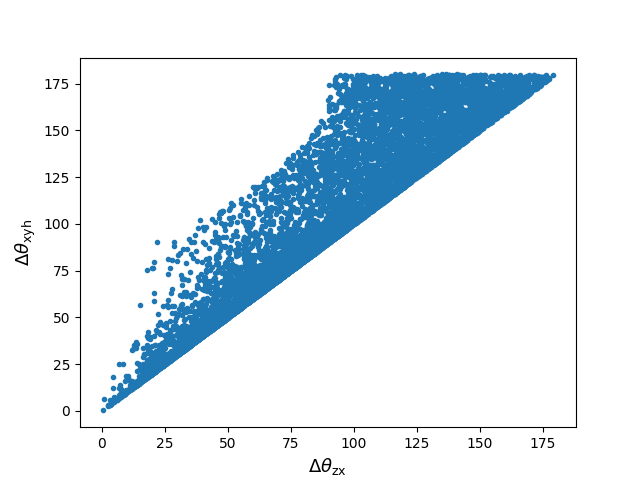
\includegraphics[width=0.65\textwidth]{figures/cmp_cmg_rot}
\caption{利用随机生成的“新、旧”指向,来对比不同转动角计算方法所给出的结果:
横轴($\Delta\theta_{\rm zx}$)是张鑫原来的计算结果,
纵轴($\Delta\theta_{\rm xyh}$)是考虑了“不产生像旋”这一限制后的计算结果。}
\label{fig:cmp_cmg_rot}
\end{figure}

%%%% CMG温度变化的建模
\subsubsection{CMG产热、散热的模型}
目前我们粗略地假设CMG机动时的产热速率、散热速率均为常数,分别记为$\alpha$,$\beta$。
另外我们假定,表\ref{tab:cmg}中每一行所给出的允许的机动方式能保证CMG的温度回归到初始的状态,
也就是在一轨的时间内,CMG的温度经历了上升、下降之后,至少能够回到开始转动前的状态。由此我们
可以列出一个不等式来,并且可以根据表\ref{tab:cmg}和表\ref{tab:trans_time}中的数据对$\alpha$与
$\beta$的关系进行限制。

从表\ref{tab:trans_time}的第一行可以推断出,望远镜指向发生改变后,至少需要70秒的时间来
进行稳定。表\ref{tab:cmg}中的每一行都有一个最大转动角度,从工程的角度来讲,只要最大角度的
转动能够实现,小一些的角度的转动必然是可行的。因此我们可以选择每一行的最大转动角(以及对应
的转动时间)来限制$\alpha$和$\beta$之间的比例关系。

\begin{figure}[h!]
\centering
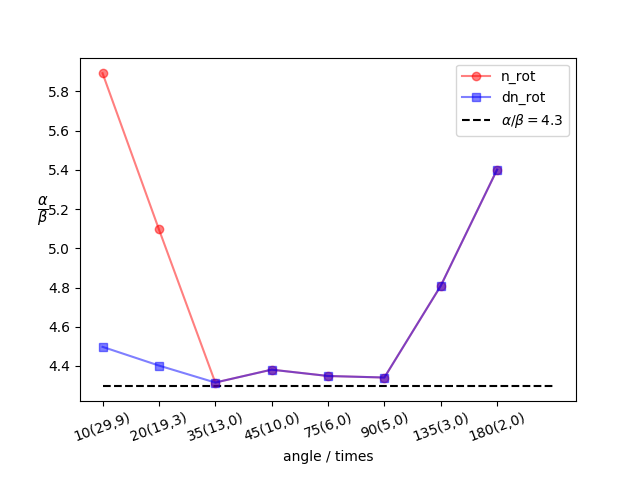
\includegraphics[width=0.65\textwidth]{figures/CMG_alpha2beta.png}
\caption{根据表\ref{tab:cmg}和表\ref{tab:trans_time}中的数据得到的CMG产热、散热系数的比值。}
\label{fig:cmg_alpha_beta}
\end{figure}

根据前面的假设,一轨时间($T_{\rm orbit}$)内的产热总量$Q_{\rm gain}$正比于机动的次数$n$和
单次机动的转动时间$T$(暂时忽略加速和减速的时间),于是有
\begin{eqnarray}
Q_{\rm gain} = n\cdot (T-70)\cdot \alpha
\end{eqnarray}
这里$T$代表的是CMG加速、匀速、减速、稳定所需的总时间,因此减去了70秒(此处暂且忽略加速、
减速转动所占的时间)。
一轨内的散热总量$Q_{\rm lost}=\beta\cdot T_{\rm orbit}$,并且必须不小于$Q_{\rm gain}$,
由此可以得到$\alpha$和$\beta$之间必须满足下列关系
\begin{eqnarray}
\frac{\alpha}{\beta} \le \frac{1}{n} \frac{T_{\rm orbit}}{T-70}
\end{eqnarray}
图\ref{fig:cmg_alpha_beta}中给出了不同转动角度情况下的$\alpha / \beta$。在35度至90度的范围内,
$\alpha / \beta$的值相比在其他范围小很多,意味着散热效率要高一些。
\RT{\heiti 因此,如果要用这个模型来检验巡天模拟中CMG的使用情况,应该假设散热效率最低的情况,
简单说就是假设$\alpha=1,\beta\simeq 1/6$。}

{\kaishu
\textbf{更新:}在发热、散热速率都恒定的假设下,可以进一步简化描述CMG转动角度与机动次数之间的关系。
在发热、散热速率恒定的假设下,可以知道机动的次数受到转动角度的限制。其实从五院提供的数据也可以看到
这一点(表~\ref{tab:cmg}中的3-6行),一轨时间内可以转过的总角度是有一个上限的(450\textdegree)。

因为转动角度等于机动时的最大角速度乘以时间(包含了加、减速时间的改正),我们需要从相关数据中推断
出最大角速度 $\omega_{\rm max}$,然后就可以根据所需的转动角度反推出机动时间,并得到有多少热量
产生。为了进行加、减速的时间改正,我们还需要知道角加速度$\Omega$,以及消除机动过程中产生的机械
振动所需的稳定时间$t_{\rm stab}$。
}

\subsection{帆板的转动}
\label{sub:panel}
从我接受这个任务开始,帆板是一直被假设为相对于望远镜镜筒是固定的。实际上,这一假设使得望远镜
在阳照区寻找可观测天区的搜索范围小于帆板可转动的情况,进而会导致搜索天区的效率下降。

\textbf{2018-8-8:}完成了在帆板可以转动($\pm 25$\textdegree)的情况下,其法线与太阳的夹角如何
计算,具体计算(其实是搜索)过程总结如下。

\MT{\heiti 首先建立一个固定在望远镜上的局部直角坐标系}。该坐标系的三个轴分别是沿着望远镜光轴的单位矢量$\bm{p}$,
垂直于望远镜所在子午圈的一个单位矢量$\bm{n}_{0}$(在不考虑帆板可以转动时,$\bm{n}_{0}$与帆板法线重合),
最后一个是帆板绕转动轴方向的单位矢量,用$\bm{A}$表示。这三个单位矢量之间有如下的关系:
\begin{eqnarray}
\bm{A}=\bm{p}\times\bm{n}_{0}.
\end{eqnarray}

\MT{\heiti 第二步是构造出以$\bm{A}$为旋转轴的旋转矩阵$\bm{R}(\bm{A},\alpha)$。}矩阵的具体
构造公式可以参考\url{https://en.wikipedia.org/wiki/Rotation_matrix}中的相关介绍。有了旋转矩阵
$R(\bm{A},\alpha)$之后,我们就可以得到转动任意角度$\alpha$后的帆板法线指向
\begin{eqnarray}
\bm{n}(\alpha) = \bm{R}(\bm{A},\alpha)\cdot\bm{n}_{0},
\end{eqnarray}
显然,当帆板没有进行转动的时候($\alpha=0$),就有$\bm{n}(0)=\bm{n}_{0}$。

\MT{\heiti 第三步是寻找使得帆板法线与太阳夹角最小时的转动角$\alpha$。}我实现的算法是从
$\alpha=-25$\textdegree 开始,以1\textdegree 的步长逐一计算$\bm{n}(\alpha)\cdot\bm{X}_{Sun}$,
直到找到最大值;如果在步进到25\textdegree 之前发现某个$\alpha$的取值已经使得
$\bm{n}(\alpha)\cdot\bm{X}_{Sun}=1$,则说明可以通过旋转使得帆板正对于太阳,此时
就直接退出搜寻的过程,减少不必要的计算。

\BT{\heiti 帆板转动计算的比较:}
这里对比一下张鑫原先实现的帆板转动算法与我重新实现的算法。
\RT{张鑫和唐怀金分别提供了一份测试程序。测试结果显示三者的计算结果一致。}


\subsection{阴影区、阳照区的判断}
在阴影区时望远镜进行观测的条件与其在阳照区时所需要满足的条件是不同的。

\subsection{曝光时间的计算}
目前的模拟对曝光时间进行了简化处理:大面积多色巡天的曝光时间为150秒,极深度多色巡天的曝光时间为250秒。


\subsection{天区划分}

天区划分与所使用的探测器的尺寸有关。

\subsubsection{探测器的相关参数}
目前假设使用的探测器为e2V公司所生产的型号290-00的CCD。单片CCD的尺寸(光敏面积)为
$92.2\text{mm}\times93.7\text{mm}$,像元数为$9216\times 9232$。经换算可知单片CCD的有效视场面积为
$0.0361743~\Box$\textdegree,30块同样尺寸的CCD拼接之后的有效视场面积约为$1.1~\Box$\textdegree
(精确值为$1.06878~\Box$\textdegree)。

\subsubsection{探测器的有效观测面积}

进行无缝光谱成像的时候,在边缘部分会有部分光谱跑出CCD的感光部分,从而导致有效的曝光面积减少。
这一效应在目前的模拟中已经包括了,所减少的有效视场宽度为点光源的光谱长度的一半。

\subsubsection{具体的天区划分方式}

\BT{\heiti 为了获得较高的信噪比,望远镜在进行曝光时应尽可能避开银盘和黄道面这样的具有很强背景光的区域。}

模拟程序在划分天区时,会根据天区的黄道坐标和银道坐标来判定是否将其选择为目标观测天区。目前的判定
方式是黄纬、银纬的绝对值需要分别大于某个阈值,并且阈值不能太大或者太小,否则会导致划分的天区面积
过大或过小,最终实际能够有效覆盖的面积反而会减少。

不过目前极深场天区的选择可以不考虑中、高纬度条件的约束,我们也选取了一些低纬度的区域。
\RT{继续补充这里的内容。。。}

\BT{詹老师提供的一个想法:如果巡天末期望远镜的使用效率降低,也就是有很多时候没有进行观测(即使
CMG的消耗处于很低的状态,能源业依旧充足),可以转而观测所划分的天区边缘地带(这些实际上不属于
选择来进行观测的天区范围)。这个想法的实现也比较的容易,但暂时还是先着手解决更主要的问题,先把
10年内能够达到的观测面积给提升上去。}

\subsection{停靠维护}
在10年的巡天内,会有4次停靠维护。五院原先提供的停靠时间共有五次(见表~\ref{tab:stoptime}),在模拟
中我们将运行时间从10年延长到10.3年,多出来的时间用于补偿最后一次停靠的时间,这样等效来看就是只有
四次停靠。

\begin{table}[h!]
\renewcommand{\arraystretch}{1}
\centering
\begin{tabular}{c|c|c}
\toprule
停靠次数 & 开始时间 & 结束时间 \\
\hline
1 & 2460131.56 & 2460205.53 \\
\hline
2 & 2460887.37 & 2460997.22 \\
\hline
3 & 2461688.66 & 2461796.99 \\
\hline
4 & 2462429.30 & 2462538.41 \\
\hline
5 & 2463166.49 & 2463275.57 \\
\bottomrule
\end{tabular}
\caption{进行停靠维护的时间表(单位:儒略日)。}
\label{tab:stoptime}
\end{table}

\RT{\heiti 另外,由于当望远镜轨道面~\footnote{望远镜的飞行轨道有一个周期约60天的进动。}与太阳
的夹角($\beta$)小于15\textdegree 时,望远镜并不观测,所以最终实际可以用于观测的时间仅有约
6.4年。如果将$\beta$角减小到10.25\textdegree,那么可以有7年的时间用于观测。}

\blankpage
%%%%%%%%%%%%%%%%%%%%%%%%%%%%%%%%%%%%%%%%%%%%%%%%%%%%%%%%%%
\section{模拟结果}

\RT{\heiti 这部分内容记录巡天编排模拟的结果,将会按照模拟进行日期的顺序来进行继续,以便于与以往的结果
进行对比。(注:本章节的内容会与章节~\ref{sec:analysis}有部分重合,主要是对模拟结果的一些简要解读。)}

\subsection{2018年7月30日}
\textbf{本次模拟的相关输入参数:}
观测天区范围选在黄纬$|B|\ge 20$\textdegree 、银纬$|b|\ge 17$\textdegree
的范围内,并且当望远镜轨道面与太阳的夹角小于15\textdegree 的时候不进行观测~\footnote{黄道坐标
用$(L,~B)$表示,银道坐标用$(l,~b)$表示。}。

\textbf{采取的权重分配策略:}
这次模拟中采取的策略包括“连续覆盖”、“小角度优先”以及“优先完成gri波段覆盖”等。另外一个对编排结果
有比较大影响的策略是“优先观测高纬度区域”。本次模拟的两组结果就分别对应于采用和不采用“优先观测
高纬度区域”策略,且最终采取该策略的那组模拟结果要更好一些。

\textbf{天区覆盖及面积统计:}
图~\ref{fig:covered_sky}和~\ref{fig:area_growth}中分别展示了最终的天区覆盖情况和有效天区覆盖面积
随时间的增长情况。模拟的结果显示,深度巡天的覆盖面积可以达到16517平方度,极深度巡天的覆盖面积
达到400平方度。

\begin{figure}[h!]
\centering
%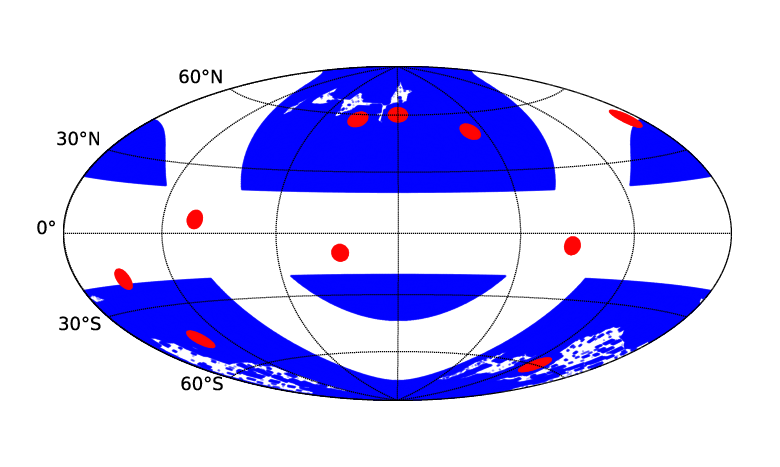
\includegraphics[width=\textwidth,angle=-90]{figures/covered_sky.png}
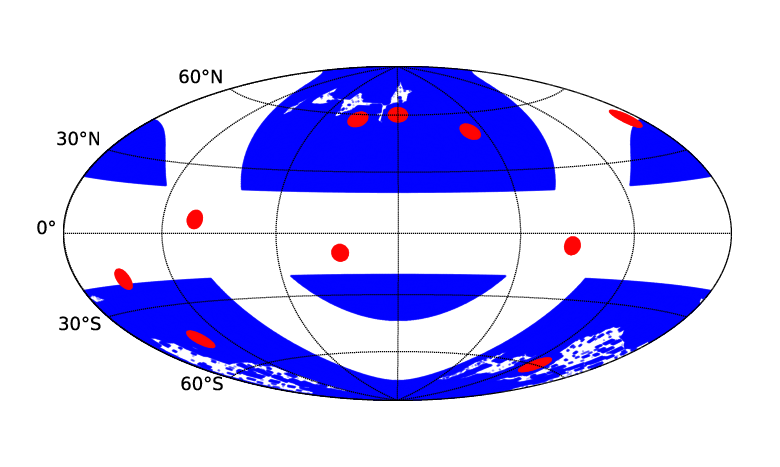
\includegraphics[width=0.8\textwidth]{figures/covered_sky.png}
\caption{10年巡天结束后的天区覆盖情况(数据来自2018年7月30日的模拟结果)。在高纬度区域仍有不少
面积未能被覆盖到,我在查看巡天末期的间隔期时发现,这些区域属于不易观测的区域,因为受到了帆板
25\textdegree 限制条件的约束(见图~\ref{fig:unobserving_debug}中所展示的绿色区域,在高纬度
区域的可观测范围比低纬度区域小很多)。}
\label{fig:covered_sky}
\end{figure}

\begin{figure}[h!]
\centering
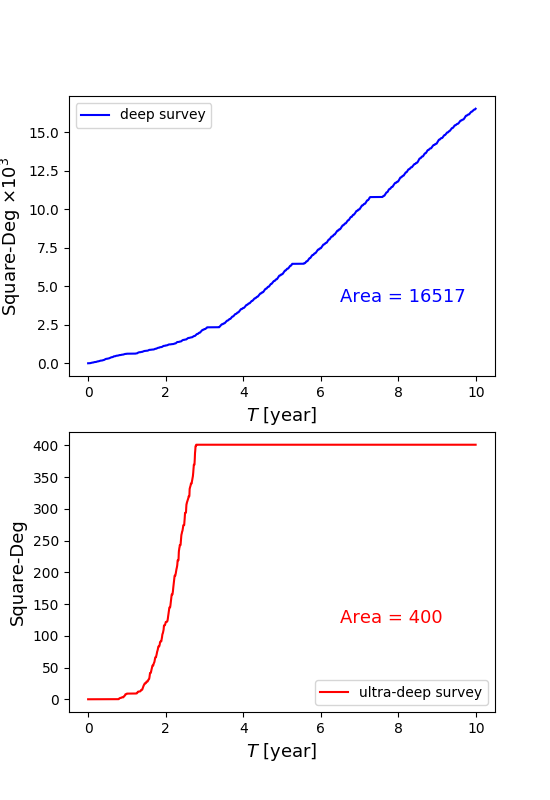
\includegraphics[width=0.6\textwidth]{figures/area_E20_b17.png}
\caption{观测天区覆盖面积的增长曲线(数据来自2018年7月30日的模拟结果)。}
\label{fig:area_growth}
\end{figure}

\subsection{2018年8月9日}
过去的这几天主要针对帆板转动做了一些工作,取消了帆板相对望远镜镜筒固定的限制。当帆板可以转动之后,
望远镜在阳照区时可以观测的范围有所扩大,出现找不到合适的可观测天区的概率也因此下降,从而巡天的效率
有所提升。


8月9日凌晨时提交了两组模拟。其中一组采取的望远镜转动方式是存在像旋问题的,这一组的结果是10年内
可以观测18300平方度+400平方度;另外一组采取的转动方式是不产生像旋的,由于这种方式所需的转动
平均而言比第一组的大,因此观测效率差不少,10年内仅能覆盖约15680平方度的天区范围,且极深场的面积
也仅有357平方度。


\RT{\heiti 现在虽然解决了一个小问题,但还有一个新的问题亟待解决:不产生像旋的转动所需要的转动角度
比较大,同时增加了CMG和时间的开销,使得最终的覆盖面积小于预期的目标。}


\subsection{2018年8月15日}
\BT{本次模拟的相关输入参数与7月30日、8月9日的基本相同,观测天区范围选在黄纬$|B|\ge 20$\textdegree 、
银纬$|b|\ge 17$\textdegree 的范围内,并且当望远镜轨道面与太阳的夹角小于15\textdegree 的时候不进行观测。
本次模拟与前面两次有所不同的是是极深场区域的选择有所改变(总面积保持不变),
具体分布见图~\ref{fig:covered_sky_0814}。}

\BT{本次模拟取消了“连续覆盖”、“优先完成gri波段覆盖”、“优先观测太阳两侧90度(经度圈)附近$\pm$25\textdegree
范围”以及“高纬度区域优先观测”等策略(对极深场观测也有部分优化,主要是增加了连续观测同一极深场天区
的权重)。总的来说,小角度的转动还是优先的,但在此基础之上进一步增加了5\textdegree 转动的权重;
在连续观测同一个区域时,因为不需要转动望远镜,因此又稍微节省了部分时间。}

望远镜的转动方式采取的是\textbf{“不产生像旋”}的方案,并且\textbf{帆板可以转动}(具体的转动方式
和角度计算见章节~\ref{sub:panel}中的介绍),使得其法线与太阳之间的夹角可以尽可能的小,保证在
阳照区的时候可以充分吸收太阳能,保证整个巡天过程中能源充足。

\textbf{天区覆盖及面积统计:}图~\ref{fig:covered_sky_0814}和~\ref{fig:area_growth_0804}中分别
展示了最终的天区覆盖情况和有效天区覆盖面积随时间的增长情况。模拟的结果显示,深度巡天的覆盖面积
可以达到16630平方度,但是极深度巡天的覆盖面积仅达到305.5平方度(主要原因是有几个极深场分布在
较高纬度,模拟进行到后期时,这些区域被观测的概率明显降低,最终导致无法完成目标;现在已经重新提
交了两组模拟,开启了高纬度优先观测的策略选项)。

目前已经完成的结果显示,取消“优先观测太阳两侧90度(经度圈)附近$\pm$25\textdegree 范围”可以
提高巡天的效率。

\begin{figure}[h!]
\centering
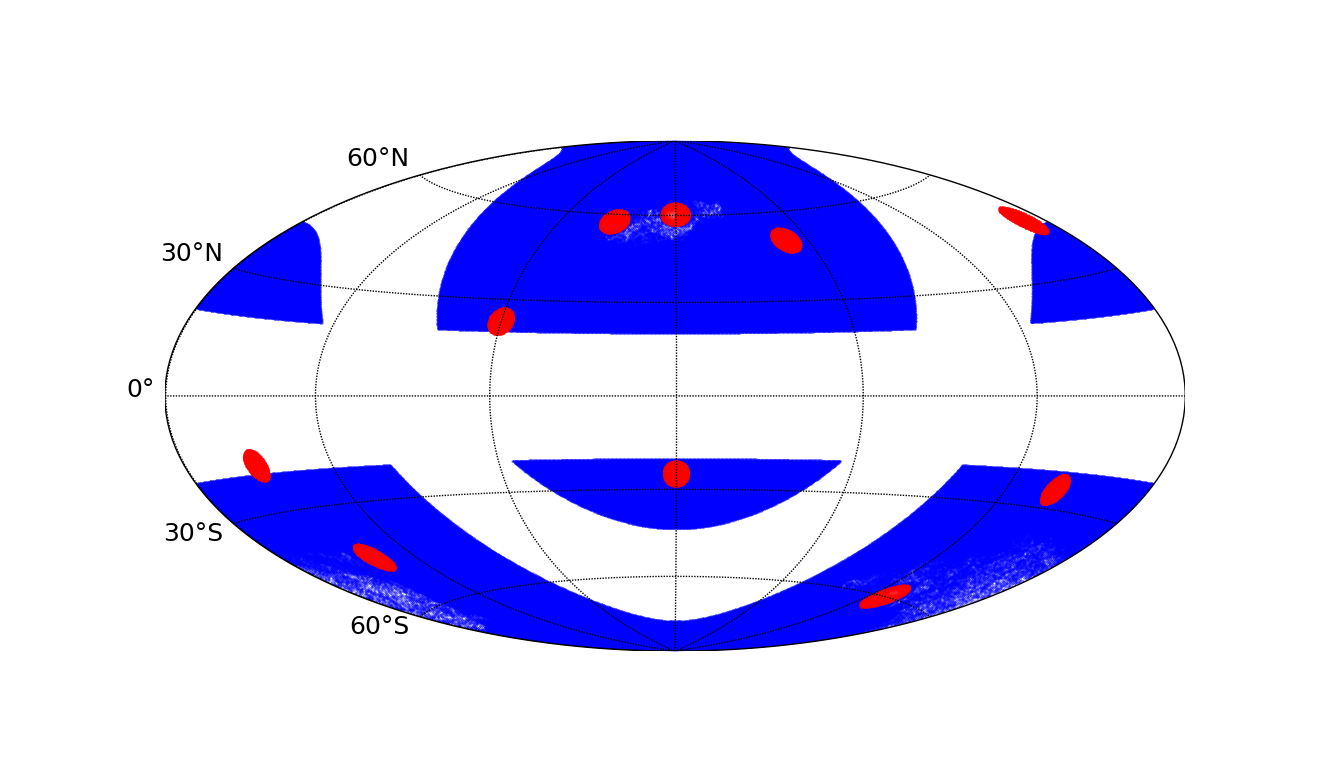
\includegraphics[width=1.3\textwidth,angle=-90]{figures/covered_sky_0814_test-A.png}
%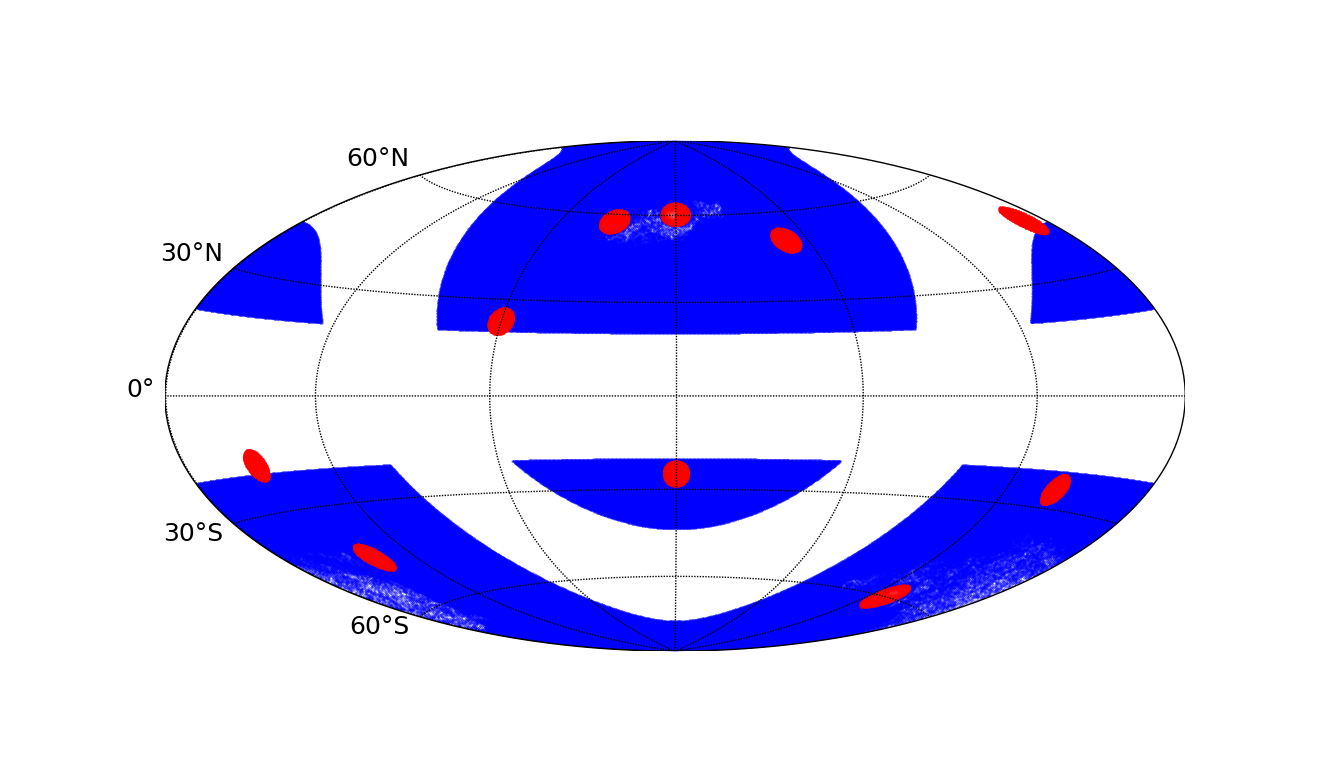
\includegraphics[width=\textwidth]{figures/covered_sky_0814_test-A.png}
\caption{10年巡天结束后的天区覆盖情况(数据来自2018年8月14日的(提交)模拟结果)。在高纬度区域
有不少天区未能被覆盖,但因为图像被缩小,不能比较清楚地显示出来。}
\label{fig:covered_sky_0814}
\end{figure}

\begin{figure}[h!]
\centering
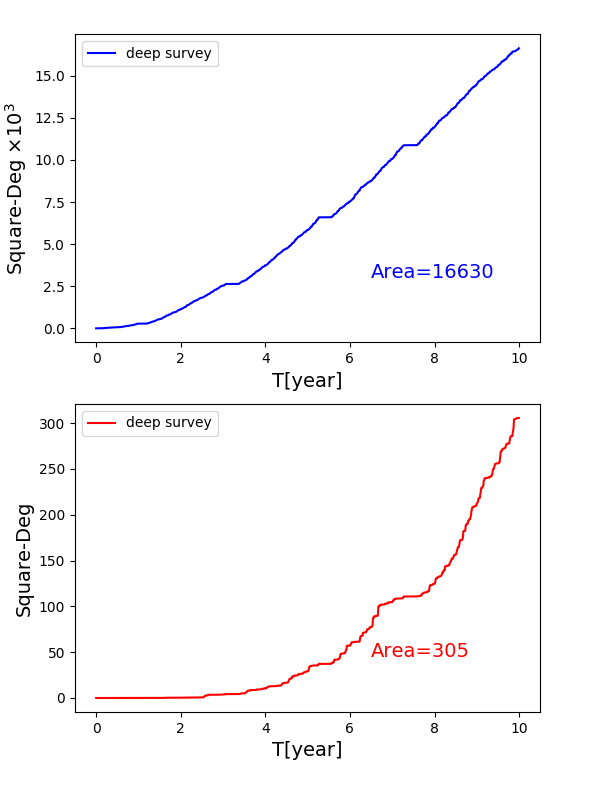
\includegraphics[width=0.6\textwidth]{figures/area_E20_b17_0814.png}
\caption{观测天区覆盖面积的增长曲线。因为有几个极深场处于较高纬度处,而这些区域又恰好是在巡天末期
时更不容易观测的区域,因此目前的模拟中还不能完成400平方度的巡天面积目标。\RT{如果将极深场选在稍微靠
边缘的区域,应该就可以在10年内完成既定目标了,但暂时还没有进行这样的模拟。}(数据来自2018年8月14日
的模拟结果)。}
\label{fig:area_growth_0804}
\end{figure}

\begin{figure}[h!]
\centering
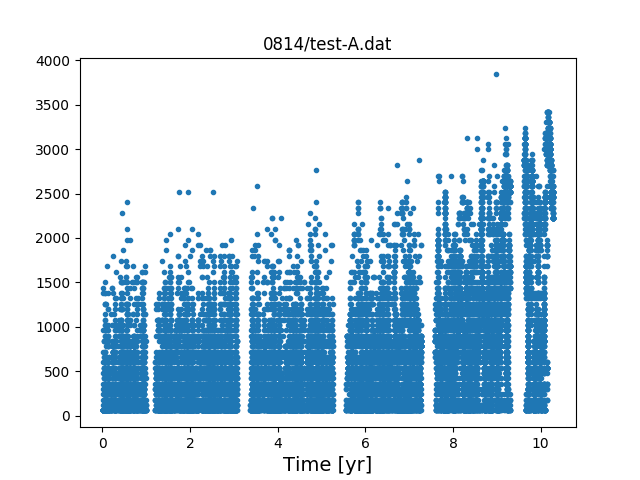
\includegraphics[width=0.65\textwidth]{figures/0814_test-A.png}
\caption{望远镜长时间不观测(间隔期)的时长在整个巡天周期内的分布情况(纵坐标单位为“秒”)。
中间5个空白处对应着5次停靠维护。与7月30日的模拟结果相比(见图~\ref{fig:time_wasted}),巡天早期的
天区覆盖效率有很大提升,但是到了7年之后,效率开始逐渐下降,甚至比7月30日的结果还要差一些。
(本图的统计结果来自2018年8月14日的模拟结果)}
\label{fig:time_wasted_0814}
\end{figure}

\subsection{2018年8月16日} \label{sec:result_2018_8_16}
8月15日提交的两组开启“优先观测高纬度”策略的模拟结果仅有很微小的提升:大面积巡天的覆盖面积从16630
平方度增加到16713平方度,而极深场的面积却从305.5平方度减少到298.89平方度。到达巡天末期时,在高
纬度区域依然有不少天区不能被很好的覆盖,且这些区域均有选定的极深场区域。直接后果就是极深场400
平方度的任务在10年内无法完成。刚才又提交了几个模拟,调整了极深场的位置,都往划分的可观测天区的
边缘靠拢。极深场的具体分布见图~\ref{fig:dist_deep_0816}。为此,我再次提交了三组模拟,模拟结果
分别输出到:
\begin{itemize}
\item test-A\_new\_deep\_positions.dat(未开启高纬度优先), 
\item test-C\_highL\_7.5yr\_new\_deep\_positions.dat(前7.5年开启高纬度优先),
\item test-C\_highL\_9yr\_new\_deep\_positions.dat(前9年开启高纬度优先)。
\end{itemize}

\begin{figure}[h!]
\centering
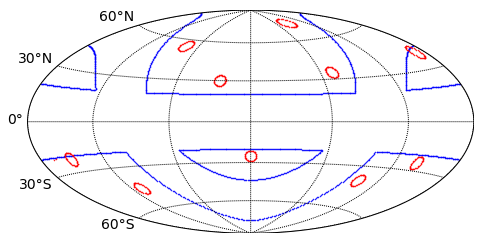
\includegraphics[width=0.75\textwidth]{figures/dist_deep_0816.png}
\caption{2018年8月16日提交的三组模拟的极深场区域的分布。图中极深场区域基本都选择在
划分的可观测天区的边缘附近,而这些边缘地带一般情况下到巡天末期都会被很完整地覆盖,因此
可以预期,这些位置的极深场最终都能够被完整地覆盖。}
\label{fig:dist_deep_0816}
\end{figure}

{\heiti 今天晚些时候在分析模拟结果时发现,“连续观测同一极深场天区”这个策略被“优先观测望远镜运动方向
的天区”破坏掉了。具体内容见章节~\ref{sec:analysis_2018_8_16}的分析;在修改了相应的代码之后,重新提交
了一组模拟,相应的结果输出到test-C\_highL\_9yr\_deep\_positions\_deep\_prior.dat(前9年开启高纬度优先)。}

\blankpage
%%%%%%%%%%%%%%%%%%%%%%%%%%%%%%%%%%%%%%%%%%%%%%%%%%%%%%%%%%

\section{限制因素分析}
\label{sec:analysis}
判定主要限制因素的办法就是直接查看模拟生成的指向序列,检查出现长时间不观测(以下简称“间隔期”)之前
望远镜的运行状况(能源和CMG的使用情况)。

目前已经找出来几种会导致望远镜长时间不观测的因素,其中主要
因素就是CMG使用过度(这种情况主要出现在巡天早起的时候)、剩下的未观测天区的数目比较少,导致即使在
各项限制条件都满足的情况下找不到可以观测的天区(这类情况主要集中在巡天末期)。在巡天中期的时候,
望远镜虽然也会出现较长时间不观测的情况,但是这些停止观测的时间长度平均而言要比早期和末期的不观测
时间长度小很多(见图~\ref{fig:time_wasted}中所展示的间隔期时长在整个巡天周期内的分布)。

\begin{figure}[h!]
\centering
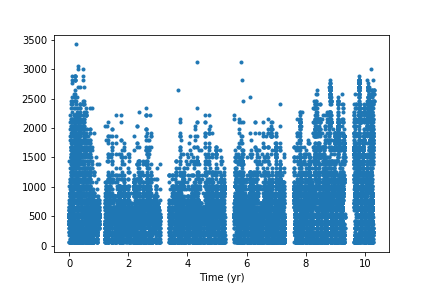
\includegraphics[width=0.75\textwidth]{figures/dT_vs_time.png}
\caption{望远镜长时间不观测(间隔期)的时长在整个巡天周期内的分布情况(纵坐标单位为“秒”)。
中间5个空白处对应着5次停靠维护。(本图的统计结果来自2018年7月30日的模拟结果)}
\label{fig:time_wasted}
\end{figure}

\textbf{指向序列的查看方法:}首先对模拟结果进行预处理,将那些望远镜长时间不观测的时间段找出来(根据
当前曝光的时刻加上曝光时间以及转动到下一次指向所需的时间,与下一次曝光开始的时刻进行比对),并排除
掉由于停靠维护、望远镜轨道面与太阳的倾角小于15\textdegree 时不进行观测的情况。找出来的这些间隔期对应
的观测时间(准确讲是间隔期的结束时间)以及间隔期的长度输出保存到文本文件中。随后根据这些间隔期的出现
的时间,定位到模拟结果中相应的位置,沿着时间的反方向将每一次曝光开始时的天区覆盖情况,太阳、月球、
地球等对可观测天区的限制情况以及是否处在阳照区(如果在阳照区,那么图上会增加一个标题用于提醒)。
在图~\ref{fig:unobserving_debug}中我展示了某个间隔期开始前的最后一次曝光与结束后的第一次曝光时的可观测
天区的情况。


\begin{figure}[h!]
\centering
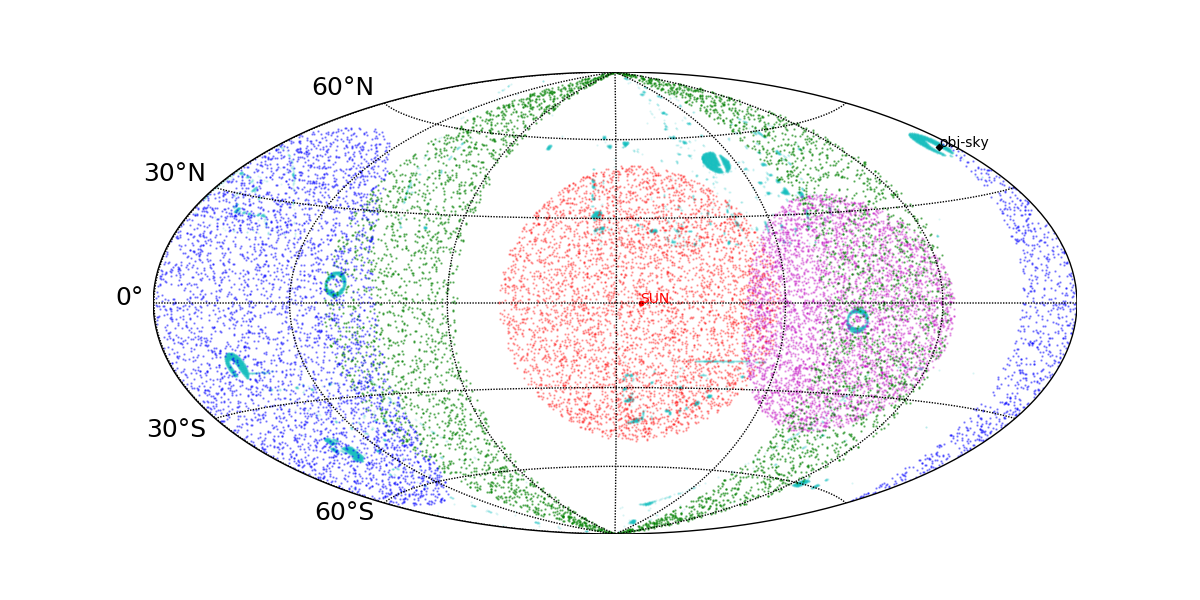
\includegraphics[width=\textwidth]{figures/xxx_1_1.png}
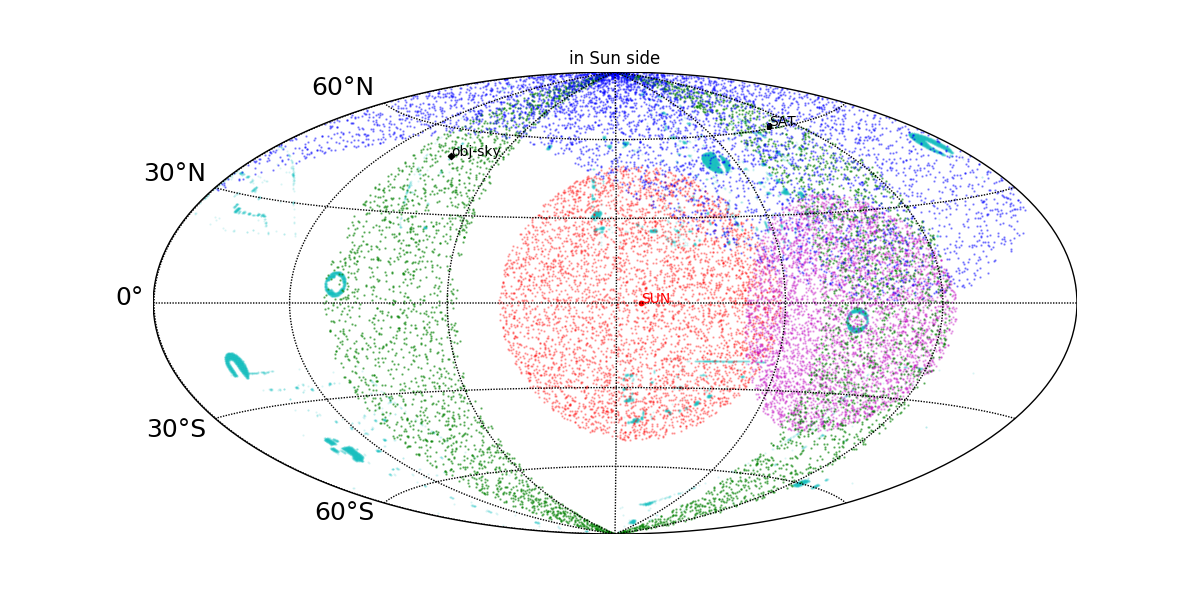
\includegraphics[width=\textwidth]{figures/xxx_1_0.png}
\caption{望远镜长时间不进行观测的间隔期的天区覆盖情况示意图(巡天进行到0.242年的时候)。\textbf{上图}是
进入间隔期前的最后一次观测指向,\textbf{下图}是间隔期结束后的第一次观测指向(观测指向用obj-sky标出)。
其中青色(cyan)表示已经被观测过的天区,红色和粉色分别表示当时受到太阳和月球的限制而无法观测的区域,绿色
区域代表的是加上太阳能帆板25\textdegree 夹角限制后所能观测的天区,最后蓝色代表的是当时望远镜的天顶角
60\textdegree 范围内的可观测区域(目前为了画图方便,这个区域并不严格与模拟运行时设定的规避地球杂散光、
地气光的限制一致)。\RT{我们还可以在该图中望远镜的位置处标出其当时的运动轨迹。}}
\label{fig:unobserving_debug}
\end{figure}

\subsection{7月30日~8月3日}
\RT{此处分析基于2018年7月30日的模拟运行结果。}

目前已经从模拟结果中分析得到一些与\textit{望远镜出现长时间不观测}有关的特征~\footnote{这里具体是指超过约
50分钟的间隔期;另外还观察到存在许多时间长度为2000秒左右的间隔期,这类间隔有着很明显的周期性,与当时
的可以观测的天区分布有着密切的关系。},并且可以将这些特征大致分为三类,与具体的观测时期有关。具体分类
包括巡天早期($\lesssim$0.5年时),巡天中期($\sim 5$年)和巡天快结束的时候($\gtrsim$9年)。

\textbf{巡天早期:}这个时期内,由于采取了“极深场优先观测”的策略,导致一轨内的观测指向很大概率地集中于
极深场,更重要的是导致了不少的大角度转动(极深场分布比较离散),最终效果就是CMG的消耗维持在一个很高
的水平(从模拟生成的序列中可以看到不少连续序列对应的CMG值都超过了0.95)。\MT{这时期望远镜不观测的
间隔期几乎都开始于要从阴影区进入阳照区的时候。在阴影区的时候,因为没有帆板25\textdegree 夹角的限制,
望远镜的指向可以更加任意,但是一旦进入阳照区,就必须要将指向转动到帆板25\textdegree 夹角所允许的范围,
这样一来就很可能需要通过一个大角度转动来实现,而此时的CMG消耗又处于很高的水平,自然这样的转动就不被
允许了,最终结果就是进入一个较长时间的等待状态。}

同时,我还在指向序列中看到了一些明显不是很优化的结果。例如,有些挨得很近的指向(属于极深场区域)其实
可以很连续地进行观测的,这样只需要很小角度的转动,不仅减少了转动所需的时间,还降低了CMG的消耗;但是
这些指向的观测却是被分开的,中间穿插了两、三次的大角度的转动。\RT{我个人觉得这与目前所采用的权重分配方案
有直接的联系。}

\textbf{巡天中期:}巡天中期出现长时间不观测的原因与巡天初期类似,不过平均而言这个时期内的间隔期长度
要显著小于巡天初期和末期(见图~\ref{fig:time_wasted}中所展示的间隔期时长在整个巡天周期内的分布)。

\textbf{巡天晚期:}CMG的往往没有被用足,此时望远镜不观测主要是因为往前一步时找不
 到合适的天区(这里的合适是指不需要经过大角度转动)。\RT{有一个想法,如果将在初期优先观测极深场的
 安排挪到后期,会不会有什么改观?}



%%%%%%%%%%%%%%%%%%%%%%%%%%%%%%%%%%%%%%%%%%%%%%%%%%%%%%%%%%
\newpage
\section{策略优化}

\RT{
需要切记,做优化的前提是对望远镜不能高效利用时间进行观测的原因有充分深刻的认识和理解!
}

\BT{目前所使用的策略还是以张鑫之前的工作为基础。2018年7月30日的模拟中使用的策略与张鑫年后跑的模拟一致。
从8月7日起,开始策略部分的调整。}

整个搜寻的策略可以根据“对候选天区进行观测时望远镜所处的境况”划分为两大类,分别是处于阳照区和处于阴影区的
时候。当望远镜处在这两个不同区域中的时候,所受到的限制条件(尤其是能源条件)有所不同,因此在制定具体的
权重分配策略时需要对这两种情况分开考虑。

\subsection{张鑫制定的权重分配策略}
有必要详细回顾一下张鑫原先制定的权重分配策略,并对这些策略进行详细的量化的检验,找到其中可能存在的
相互冲突的部分,最终提出解决方案。

\subsection{策略制定的再思考!}


\subsection{目前已经尝试过的改动}
我前阵子尝试过对策略进行了一些改动,主要是对“极深场部分的优先观测策略”和“连续观测策略”进行了调整,
能够使得最终的有效巡天面积增加近1000$\Box$\textdegree 。

\subsubsection{2018-8-7}

提交了两组模拟,策略部分主要的修改(相比张鑫的策略)是将“极深场优先观测”
挪到根据CMG转动角度进行权重分配的部分了。如此一来就直接把出现在早期的长时间不观测的情况大大减少了,
并且根据之前尝试的结果,最终的大面积巡天可以达到17500$\Box$\textdegree 的要求,但是“极深场”的面积
还没有达标,于是这一次增加了一个从8.5年开始优先观测极深场的策略。\RT{这一改动可以等效地看作是将原先
的尽可能早地完成极深场观测的计划挪到整个观测周期的末尾阶段了。}
\BT{另外一个改进就是,当对极深场的同一天区进行重复观测时,因为不需要进行转动,此时的CMG消耗没有
任何的增加,也不需要进行稳定过程,所以又可以节省一部分时间,目前假设可以节约30秒(小于1\textdegree
的转动+稳定所需的总时间为80秒,CCD数据的读出需要40秒;此处我假定需要50秒,将CCD刷新的时间
也包含在内)。}

本次的两组模拟的不同之处是,一组的高纬度观测策略持续到5年的时候,而另一组持续到8.5年的时候。
同时,这两组的“连续观测策略”的使用时间被限制在3年至8年之间。

傍晚的时候又提交了一个天区划分稍微更大的模拟(E=19,b=17),其余条件分别是“高纬度优先策略”持续到
8.5年,“连续观测策略”从3年到8年之间,不考虑大角度转动的“极深场优先”也是从第8.5年开始。

刚刚修正了主函数结束部分的一个释放内存的bug,这个bug可能导致最后有部分结果不能正常输出到文件中去
(在服务器上运行时),\RT{大约有2天的曝光序列被浪费掉}。

在修正了这个bug之后,又提交了两组模拟(E=19,E=20)。其余运行条件分别是“高纬度优先策略”持续到8.5年,
而“连续观测策略”改为在5年到8年之间,不考虑大角度转动的“极深场优先”依旧是从第8.5年开始。

\subsubsection{2018-8-8}
实现了允许帆板转动的代码。

基本想法如下:首先利用对称性可以将不同纬度上旋转帆板的问题都简化成当望远镜处在黄道面上时的帆板转动问题;
尽管现在帆板可以绕轴旋转正负25度,引入一个假想的还是固定的帆板可以进一步简化问题。原先帆板固定时,
望远镜搜寻可观测天区的范围被限制在一个$\pm$25\textdegree 的带中,现在帆板可以转动了之后,与太阳的
夹角就可以借助转动来消除了。

\RT{上面所描述的基本想法其实是错误的,因为当望远镜指向黄赤道与指向其他方向时,帆板转动对于改变
其法线与太阳夹角的效果是不一样的。}傍晚的时候重新构思了如何实现帆板的转动,先是用python做了
简单的模拟,一步一步地计算了当帆板绕轴旋转时,帆板法线与太阳的夹角的余弦值是如何变化的。依据
所画的图来看,计算是没有问题的。随后,将这部分算法移植到模拟程序中去,并通过一番测试,检查和
修复了部分bug。最后提交了两组模拟,一组使用的是旧的望远镜转动,一组是我后来实现的可以保证不
产生像旋的转动。从最初的情况来看,有一定的希望可以达成10年内完成$17500\Box$\textdegree 的目标。
\RT{8月9日-10日的结果显示,在采用张鑫实现的望远镜转动方式的前提下,放开帆板旋转这个限制之后,
确实是可以在10年内完成目标,并且最终面积可以超过$18300\Box$\textdegree。但是当使用不产生像旋
的转动方式之后,要想在10年内完成目标还很困难,目前的模拟才只做到$15500\Box$\textdegree。}

\subsubsection{2018-8-14}
现在是凌晨1点半,刚刚修改了极深场区域的选择,几乎全部与大面积巡天的区域重合,只有少部分处在
边界的位置。这次模拟取消了所有低纬度区域的极深场观测,并且取消了“连续观测策略”和强制性的“极深场
优先策略”。依旧是一次提交了两个模拟,其中一个面积比另外一个大一些。睡觉去了。。。

(晚上11点)刚刚完成了策略部分的调整,重点调整了当天区变化方向和望远镜的运动方向一致时权重有所
增加的策略。这相比张鑫原先的做法更精细了一些,原先只要两个“位移矢量”的点积大于零就好,而现在则
是按照点积的具体数值来进行权重的调整。另外,也调整了初始权重的数值,由原先的100改为10000。
在根据CMG转动角度分配权重的部分,采用了一个高斯函数来增加(对应的是数值上的减小)5度转动的
权重。这样一来会打破原先预期的小角度转动策略。最后,我还取消了阳照区时优先观测太阳两侧(经度)
90度附近的正负25度内的区域这样一个设置。

这次的模拟中还取消了以下几个权重分配策略:1)高纬度优先;2)连续覆盖;3)gri波段优先。

\subsubsection{2018-8-15}
今早起来查看昨天提交的模拟,结果改善了很多。策略改动之后,搜索天区的成功率得到了很大的改善。
目前模拟还未结束,但是相比之前的一组模拟,在9.6年左右,就已经完成了54万次的曝光,而没改动
策略之前,54万这个数字需要等到模拟结束之后都无法达到!这次的模拟运行在前8年都有着很高的效率,
但是之后效率还是开始下降了,毕竟实现划分的观测区域的边缘部分早早地就被全部覆盖了,剩下的未
观测区域相互之间离得比较远,因此大角度转动的次数开始逐渐增加,随之而来的就是每轨的观测次数
急剧下降。

中午与唐怀金讨论和对比了一下在帆板可以转动的情况下,帆板法线与太阳夹角的计算。讨论过程中意识
到自己实现的算法里没有考虑到一种可能会出现的情况。最初在确定法线的时候,法线实际上有两个可能的
方向,应该首先确定那个方向是指向太阳的,然后再将其确定为帆板法线;随后再去通过旋转矩阵来寻找
最小的夹角。现在已经将这个漏掉的判断加入到代码中,并提交了一个新的模拟,其结果输出到
0814/test-B.dat。

前面已经提到,到了后期时(8年左右),搜寻观测天区的效率下降。于是又提交了两组使用高纬度优先
策略的模拟,分别在前7.5年和9年内,尽可能观测高纬度的,这样使得划分的天区的边缘地带有不少面积
可以留到后期进行观测。这两组模拟的结果输出到0804/test-C\_highL\_7.5yr.dat和
0804/test-C\_highL\_9yr.dat。


\subsubsection{2018-8-16} \label{sec:analysis_2018_8_16}

今天的结果显示,开启“高纬度优先观测”策略对结果没有带来明显的改进,并且最终还是有不少高纬度
区域不能很好地被覆盖(见章节~\ref{sec:result_2018_8_16}对结果的描述)。

检查了一遍模拟结果,发现没有出现预期的连续观测同一极深场的情况。仔细检查了策略之后发现,
“优先观测与望远镜飞行方向一致的天区”这一设置破坏了“优先观测同一极深场区域”这条策略。代码
中权重是按照下面的方式去设置的:
\begin{eqnarray}
\text{weight} = \text{weight} - 1000\times dp,
\label{eq:weight_dp1}
\end{eqnarray}
其中$dp$是望远镜飞行方向与两个天区的位置矢量差的点积(经过归一化)。当$dp$的值接近于1时,
就表示新的天区指向相对上一次观测的指向的位置与望远镜的飞行方向一致;反之,当$dp$的值接近于
-1时,则表示两个方向相反。这里$dp$的具体数值直接控制了权重的大小,与张鑫之前只根据$dp$的
符号来修改权重的做法不同。

如果将方程~\eqref{eq:weight_dp1}修改为下面的形式,“连续观测同一极深场天区”的策略就会有效:
\begin{eqnarray}
\text{weight} = \text{weight} - 1000\times dp\times (*\text{id} ~!= ~\text{s\_id}),
\label{eq:weight_dp2}
\end{eqnarray}
其中$*\text{id}$和$\text{s\_id}$分别表示上一次观测天区的id和当前候选观测天区的id。

另外,新增加的5\textdegree 转动优先的策略也干扰到了对极深场同一天区的连续观测,因此现在
将5\textdegree 转动优先的权重分配代码与极深场同一天区连续观测权重分配代码用if-else分隔开,
在可以连续观测时,5\textdegree 转动优先权重分配就失效。

%%%%%%%%%%%%%%%%%%%%%%%%%%%%%%%%%%%%%%%%%%%%%%%%%%%%%%%%%%
\newpage
\section{模拟结果的检验}
目前已经完成了几何限制、CMG限制的检验,还剩下能源限制、SAA限制未完成。

\subsection{检验程序中各项限制条件的设置}
该检验程序中“限制条件”的实现以编排模拟程序为基础,但在相应的地方加入了改进。下面的内容对检验程序中
“限制条件”的具体实现进行逐一说明,并与\textbf{目前}所使用的编排模拟程序中的算法进行比较。

\begin{itemize}
\item CMG温度限制条件

\item 太阳:直接计算目标天区的指向与太阳位置矢量之间夹角的余弦值,如果结果小于$\cos(50\textdegree)$,
则表示通过检验。(注:仅当望远镜处于阳照区的时候才对这一条限制条件进行验证)

\item 月球:直接计算目标天区的指向与月球位置矢量之间夹角的余弦值,如果结果小于$\cos(40\textdegree)$,
则表示通过检验。

\item 地球:该条限制的检验过程中加入了太阳张角、蒙气差的影响,比目前的编排模拟程序中采取的限制
要严格一些。现在检验程序中采用的算法由唐怀金提供。

\item SAA:该限制条件的检验暂未完成。

\item 帆板法线与太阳的夹角:编排模拟的结果中有该夹角的信息。直接查看结果后发现,有约$2.8\%$的结果
中(阳照区)会出现夹角大于25度的情况。经查看后发现,这些结果都对应于望远镜从阴影区飞行到阳照区的时候。
\BT{具体原因是,目前编排模拟程序在搜索候选观测天区的时候,首先根据上一次曝光结束时(少数情况下由于
飞跃SAA上空,该时间会往后推移)望远镜是否在阳照区来决定要做哪些具体的限制条件判断。因此,在某些情况
下,望远镜正处于要进入阳照区的时刻,限制条件中就不包括检验帆板法线与太阳夹角;在输出搜寻的候选观测
天区的信息前,程序中再一次对是否处于阳照区进行判断,这时就会发现望远镜在曝光的时候已经从阴影区跑到了
阳照区,但实现没有进行帆板法线限制条件的筛选,所以就出现了夹角大于25度的情况。}\GT{\heiti 鉴于模拟
结果中只有很小比例的曝光序列不满足帆板法线条件的限制,暂时可不考虑改进这部分的条件判断,认为检验通过。}
\end{itemize}

%%%%%%%%%%%%%%%%%%%%%%%%%%%%%%%%%%%%%%%%%%%%%%%%%%%%%%%%%%
\newpage
\section{代码优化}
\RT{这部分内容主要是针对具体代码实现的一些细节上的考虑,等到策略优化达到一定的目标以后再去进行代码的优化,
提高运行的速度。}

\subsection{代码重构}

%%%%%%%%%%%%%%%%%%%%%%%%%%%%%%%%%%%%%%%%%%%%%%%%%%%%%%%%%%
\newpage
\appendix
\section{详细参数设置}
这部分内容是对模拟程序的参数文件中各项参数的详细说明。值得注意的是,在目前的版本中,下面列出来的
部分参数已经不再使用(红色标记);同时,也有部分参数是我后来新增加的(蓝色标记)。

\begin{itemize}
\item  $\rm START\_TIME$ ~ 巡天开始的时间
\item  $\rm END\_TIME$ ~ 巡天结束的时间
\item $\rm JPL\_TIME$ ~jpl星历数据文件名
\item $\rm RESULT\_FILE$ ~巡天编排模拟结果的输出文件名
\item \RT{$\rm STATUS\_FILE\_IMG$} ~中间状态的输出文件名
\item \RT{$\rm DEEP\_AREA$} ~深度巡天面积目标值
\item \RT{$\rm ULTRALDEEP\_AREA$} ~极深度巡天面积目标值
\item \RT{$\rm STATUS\_INTVAL$} ~输出中间状态的时间间隔

\item $\rm CCD\_X$ ~划分天区时假设的CCD的X方向有效视场大小
\item $\rm CCD\_Y$ ~划分天区时假设的CCD的Y方向有效视场大小
\item \RT{$\rm CCD\_X\_DEEP$}~
\item $\rm CCD\_OVERLAP\_X$~划分天区时假设的CCD在X方向重叠的宽度
\item $\rm CCD\_OVERLAP\_Y$~划分天区时假设的CCD在Y方向重叠的宽度
\item \RT{$\rm CCD\_OVERLAP\_DEEP$}~
\item $\rm SUN\_POINT\_ANGLE$~太阳与望远镜光轴的夹角
\item $\rm MOON\_POINT\_ANGLE$~月球与望远镜光轴的夹角
\item $\rm SUN\_PANEL\_ANGLE$~帆板面法线与太阳的夹角
\item $\rm PANEL\_TRANSE\_ANGLE$~帆板可以转动的角度

\item $\rm POINT\_EARTH\_LLIMB\_ANGLE\_MAX$~望远镜光轴与地球亮边夹角的最大值
\item $\rm POINT\_EARTH\_LLIMB\_ANGLE\_MIN$~望远镜光轴与地球亮边夹角的最小值
\item $\rm POINT\_EARTH\_DLIMB\_ANGLE$~望远镜光轴与地球暗边的夹角
\item $\rm EXTIME\_ULTRAL\_DEEP$~极深场区域的曝光时间
\item $\rm EXTIME\_DEEP$~深度巡天的曝光时间
\item $\rm EXTIME\_SPEC$~光谱巡天的曝光时间
\item \RT{$\rm EXTIME\_MIN$}~

\item $\rm RANGE\_NORTH\_SEMISPHERE\_N$~划分天区时北半球的最高黄纬
\item $\rm RANGE\_NORTH\_SEMISPHERE\_S\_IMG$~~划分天区时北半球的最低黄纬
\item $\rm RANGE\_SOUTH\_SEMISPHERE\_S$~~划分天区时南半球的最高黄纬
\item $\rm RANGE\_SOUTH\_SEMISPHERE\_N\_IMG$~~划分天区时南半球的最低黄纬
\item $\rm Low\_Galaxy\_Img$~划分天区时的银纬最低值
\item $\rm Galaxy\_B\_Sec\_Low$~低银纬阈值,目前设置为25\textdegree
\item $\rm Ecliptic\_Lat\_Sec\_Low$~低黄纬阈值,目前设置为25\textdegree

\item $\rm \BT{BETA\_ANGLE}$~望远镜运行轨道面与太阳的夹角
\item $\rm \BT{HIGH\_LATITUDE\_PRIOR\_TIME}$~高纬度优先策略的有效时间(从巡天开始算起,单位:年)
\end{itemize}

\section{帆板的相关参数}
\label{sec:panel_params}
\RT{(这部分内容摘自某内部文件)}
$30\%$转换效率为地面实验室25\textdegree $C$条件下太阳电池片的标称值,
在轨情况受电池片组合匹配、紫外辐照、静电泄漏等因素影响,发电能力损失$8\%$。太阳翼在轨工作温度在
100\textdegree 左右,功率损失约$22\%$。

10年寿命考虑空间辐照的影响,性能衰减$7\%$。

阳照区内,要求帆板发电能力同时满足7500W负载供电需求和电池充电需求,考虑布片系数0.87、可靠性
冗余、蓄电池充放电损失,$75m^2$帆板的余量较小。

光学舱系统姿态稳定度目前按照0.01的帆板结构阻尼开展方案阶段仿真,正在组织能源功能按$0.02\sim 0.03$
的结构阻尼开展帆板方案优化。

后续一体化设计,平台和光学设施可结合产品继续优化整舱功耗,帆板面积和刚度不会有量级变化。

\section{模拟中还未考虑到的细节问题}

\subsection{望远镜转动过程中太阳能帆板的发电问题}




\end{document}
